% Time-stamp: <2022-11-07 11:50:04 A13258Q>
% Romain Lafarguette 2020, https://romainlafarguette.github.io/

%% ---------------------------------------------------------------------------
%% Preamble: Packages and Setup
%% ---------------------------------------------------------------------------
% Class 
\documentclass{beamer}

% Theme
\usetheme{Boadilla}
\usecolortheme{dolphin}
%\setbeamertemplate{headline}{} % Remove the top navigation bar

% Font and encoding
\usepackage[utf8]{inputenc} % Input font
\usepackage[T1]{fontenc} % Output font
\usepackage{lmodern} % Standard LateX font
\usefonttheme{serif} % Standard LateX font

% Maths 
\usepackage{amsfonts, amsmath, mathabx, bm, bbm} % Maths Fonts

% Graphics
\usepackage{graphicx} % Insert graphics
\usepackage{subfig} % Multiple figures in one graphic
\graphicspath{{/../static/img}{/../static/diagrams}}

% Layout
\usepackage{changepage}

% Colors
\usepackage{xcolor}
\definecolor{imfblue}{RGB}{0,76,151} % Official IMF color
\setbeamercolor{title}{fg=imfblue}
\setbeamercolor{frametitle}{fg=imfblue}
\setbeamercolor{structure}{fg=imfblue}

% Tables
\usepackage{booktabs,rotating,multirow} % Tabular rules and other macros
%\usepackage{pdflscape,afterpage} % Landscape mode and afterpage
%\usepackage{threeparttable} % Split long tables
\usepackage[font=scriptsize,labelfont=scriptsize,labelfont={color=imfblue}]{caption}

% Import files
\usepackage{import}

% Appendix slides
\usepackage{appendixnumberbeamer} % Manage page numbers for appendix slides

% References
\usepackage{hyperref}

% A few macros: environments
\newenvironment{wideitemize}{\itemize\addtolength{\itemsep}{10pt}}{\enditemize}
\newenvironment{wideenumerate}{\enumerate\addtolength{\itemsep}{10pt}}{\endenumerate}

\newenvironment{extrawideitemize}{\itemize\addtolength{\itemsep}{30pt}}{\enditemize}
\newenvironment{extrawideenumerate}{\enumerate\addtolength{\itemsep}{30pt}}{\endenumerate}

% Remove navigation symbols and other superfluous elements
\setbeamertemplate{navigation symbols}{}
\beamertemplatenavigationsymbolsempty

%\setbeamertemplate{note page}[plain]
\hypersetup{pdfpagemode=UseNone} % don't show bookmarks on initial view
\setbeameroption{hide notes}

% Institute font
\setbeamerfont{institute}{size=\footnotesize}
\DeclareMathSizes{10}{9}{7}{5}  

%% ---------------------------------------------------------------------------
%% Title info
%% ---------------------------------------------------------------------------
\title[Advanced Models]{Advanced Models in Forecasting}
\author[R. Lafarguette]{Romain Lafarguette, Ph.D.}
\institute[IMF]{ADIA Quant \& IMF External Consultant\thanks{\scriptsize{\emph{This training material is the property of the International Monetary Fund (IMF) and is intended for use in IMF courses. Any reuse requires the permission of the IMF.}}}}

\date[STI, 08 Nov 2022]{Singapore Training Institute, 08 November 2022}

\titlegraphic{
    \begin{figure}
    \centering
    \subfloat{{
\includegraphics[width=2cm]{../static/img/imf_logo}}}%
    \end{figure}
}

% Slide between sections
\AtBeginSection[]
{
    \begin{frame}
        \frametitle{Table of Contents}
        \tableofcontents[currentsection]
    \end{frame}
}

%% ---------------------------------------------------------------------------
%% Title slide
%% ---------------------------------------------------------------------------
\begin{document}

\section{Distributional Forecasts and Prediction Intervals}
\begin{frame}{From Point Forecasts to Distributional Forecasts}

  \begin{wideitemize}
    \item A forecast $\hat{y}_{T+h|T}$ is (usually) the mean of the conditional distribution: $Y_{T+h} | Y_1, \dots Y_T$
    \item Most models produces Gaussian distributed forecast
    \item Because models assumes Gaussian residuals: remember that the residuals are the stochastic components that are determining the distribution of both the estimators and the forecasts
    \item The forecast distribution describes the probability to forecast any future value
  \end{wideitemize}

  %TODO: add a chart
    
\end{frame}


\begin{frame}{Distributional Forecasts}

  Assuming the \textbf{residuals are uncorrelated} with variance $\sigma^2$, and with an estimate $\hat{\sigma^2}$

  \begin{alertblock}{Model Typology}
    \begin{wideitemize}
      \item \textbf{Mean:} $Y_{T+h|T} = \mathcal{N}(\overline{Y}, (1+\frac{1}{T})\hat{\sigma^2})$
      \item \textbf{Naive:} $Y_{T+h|T} = \mathcal{N}(Y_T, h\hat{\sigma^2})$
      \item \textbf{Seasonal Naive:} $Y_{T+h|T} = \mathcal{N}(Y_{T+h-m(k+1)}, (k+1)\hat{\sigma^2})$
      \item \textbf{Drift:} $Y_{T+h|T} = \mathcal{N}(Y_{T} +\frac{h}{T-1}(Y_T - Y_1), h\frac{T+h}{T}\hat{\sigma^2})$
    \end{wideitemize}
  \end{alertblock}

\medskip

\begin{wideitemize}
  \item where $k$ is the integer part of $\frac{h-1}{m}$
  \item Note that when $h=1$ and $T$ is large, these all give the same approximate variance $\hat{\sigma^2}$
\end{wideitemize}

\end{frame}



\begin{frame}{Prediction Intervals}
  \begin{block}{Definition}
      A prediction interval gives \textbf{a region} within which we expect $Y_{T+h}$ to lie with \textbf{a specified probability}
  \end{block}

\medskip
  
  \begin{wideitemize}
  \item Assuming that the forecasting errors are normally distributed, then a 95\% prediction interval is:
    \begin{equation*}
      Y_{T+h|T} \pm 1.96 \hat{\sigma_h}
    \end{equation*}
  \item where $\hat{\sigma_h}$ is the standard deviation of the h-step distribution
  \item when $h=1$, $\hat{\sigma_h}$ can be estimated from the residuals  
  \end{wideitemize}  
\end{frame}


\begin{frame}
  \frametitle{Prediction Interval Fit}
     \makebox[\linewidth]{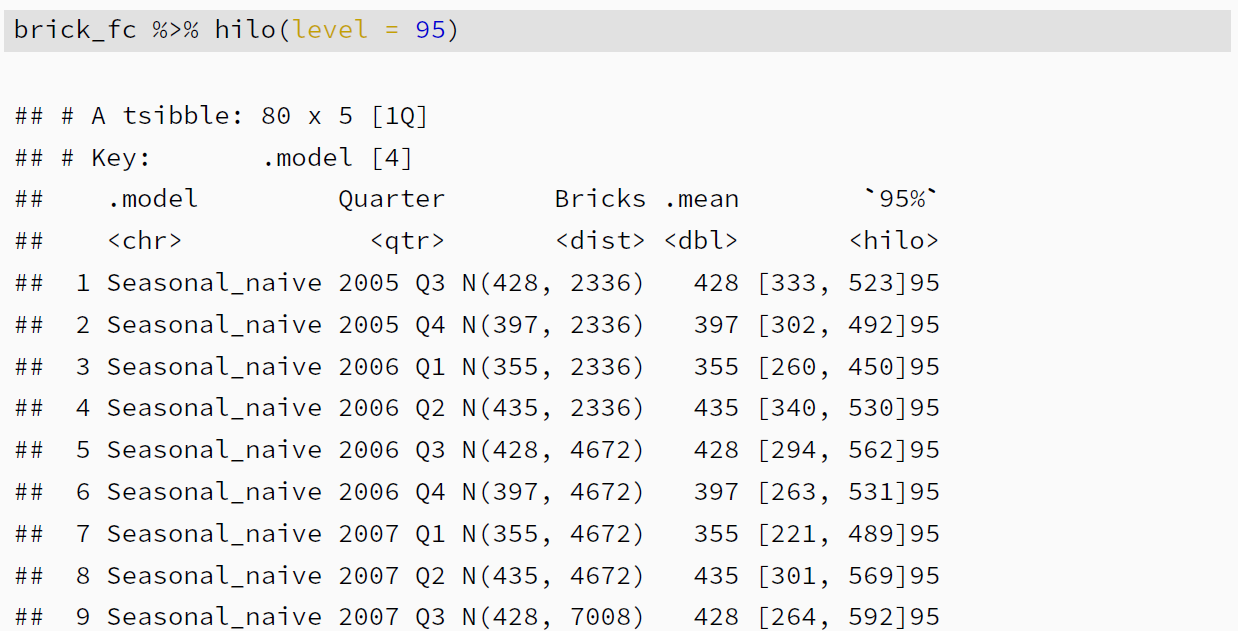
\includegraphics[width=0.95\paperwidth]{../static/course_3_img/prediction_interval.PNG}}  
\end{frame}


\begin{frame}{Why Prediction Intervals Matter}
  \begin{wideitemize}
    \item \textbf{Point forecasts are often useless without a measure of uncertainty} (such as prediction intervals)
    \item Prediction intervals require a \textbf{stochastic model} (with random errors, etc.)
    \item For most models, prediction intervals get wider as the forecast horizon increases
    \item The degree of confidence (the probability) impacts the width of the prediction interval
    \item Usually too narrow due to unaccounted uncertainty: pay attention
  \end{wideitemize}  
\end{frame}


\begin{frame}
  \frametitle{Difference between Confidence Interval and Prediction Interval}
  \begin{wideitemize}


 \item A confidence interval informs about where the true parameter of a model can be
   \begin{itemize}
     \item \textbf{Confidence interval quantifies the uncertainty about the model}, or the distance between the model and reality
     \item Confidence interval are associated with a wide range of parameters, values, etc.
     \item They inform about how the model represents well the reality
     \item Wide confidence intervals are associated with a less accurate model, and/or a very volatile model
   \end{itemize}

    
  \item The prediction interval predicts in what range a future individual observation will fall
    \begin{itemize}
      \item \textbf{Prediction interval quantifies the uncertainty about the future}, or the distance between today and the future
      \item Prediction interval are not about the parameters of the model, but about the dependent variable ($y_t$)
      \item The problem is that prediction intervals tend to neglect the uncertainty about the parameters used to generate the forecasts...
    \end{itemize}   
  \end{wideitemize}
  
\end{frame}


\begin{frame}
  \frametitle{Difference between Confidence Interval and Prediction Interval}
     \makebox[\linewidth]{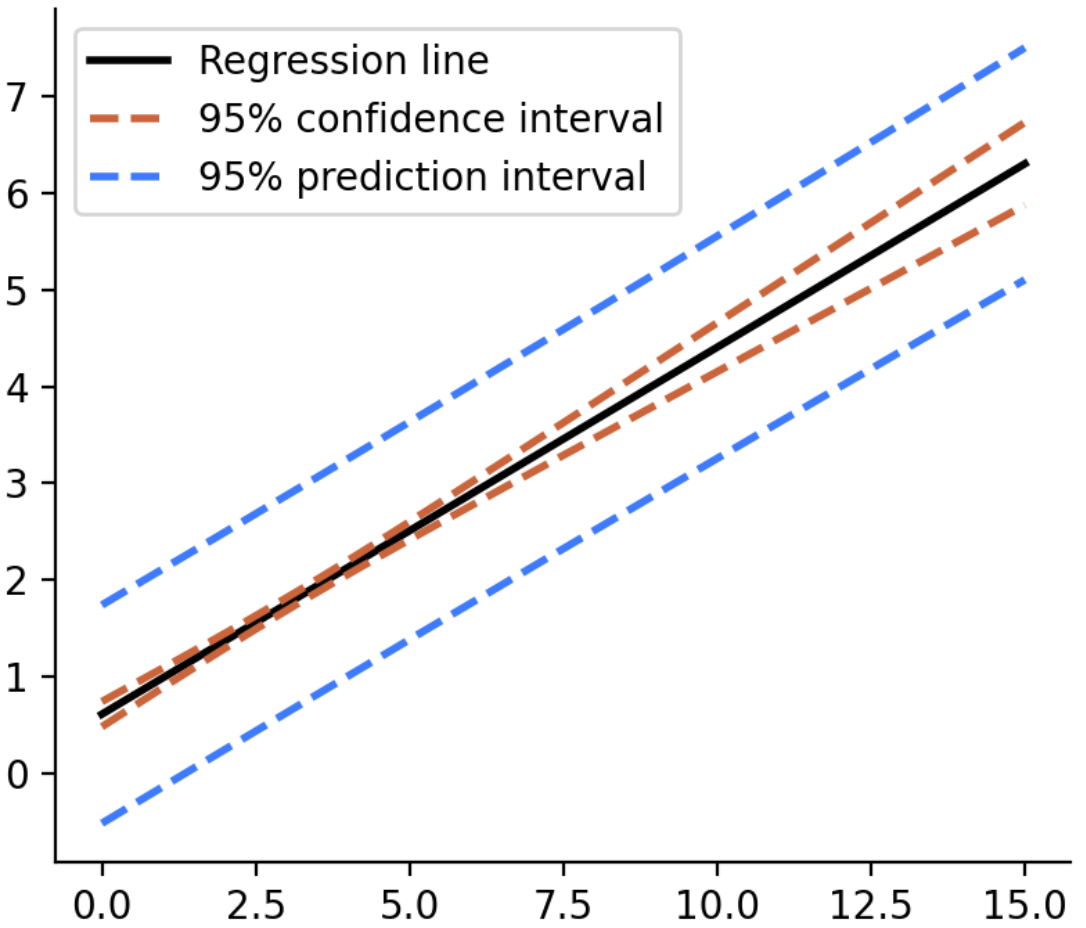
\includegraphics[width=0.75\paperwidth]{../static/course_3_img/pi_ci.png}}  
\end{frame}


\section{Evaluating Forecast Accuracy}

\begin{frame}{Fitting and Forecasting}

  \begin{alertblock}{Be careful}
    \textbf{A model that fits the data well (in sample) might not necessarily forecast well}
  \end{alertblock}

  \medskip
  
  \begin{wideitemize}
    \item A perfect in-sample fit can always be obtained by using a model with with enough parameters
    \item Over-fitting a model to data is just as bad as failing to identify a systematic pattern in the data
    \item Need to split the model between 
    \item The test set must no be used to \emph{any} aspect of model development or calculation of forecasts
    \item Forecast accuracy is only based on the test set
  \end{wideitemize}  
\end{frame}

\begin{frame}
  \frametitle{Train and Test Set}
     \makebox[\linewidth]{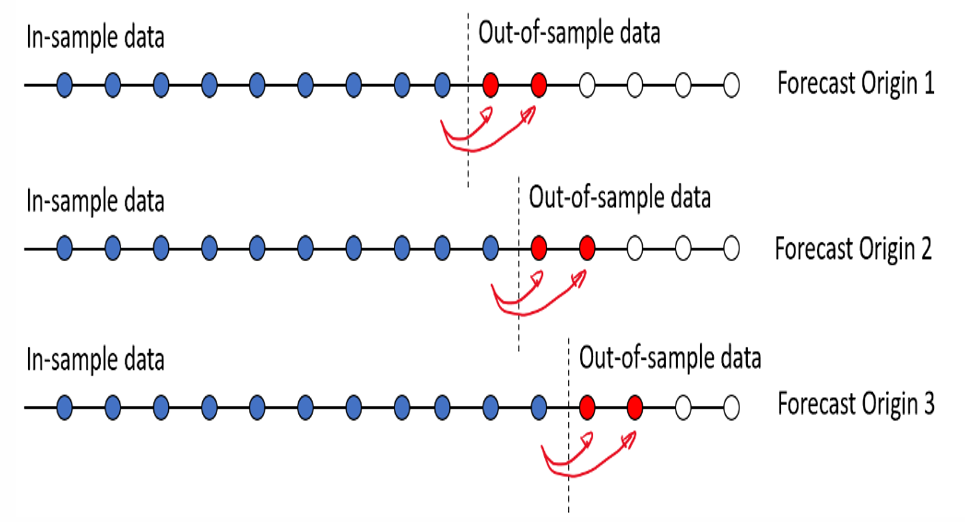
\includegraphics[width=0.95\paperwidth]{../static/course_3_img/in_sample_out_sample.PNG}}  
\end{frame}

\begin{frame}
  \frametitle{Underfit, Optimal, Overfit}
     \makebox[\linewidth]{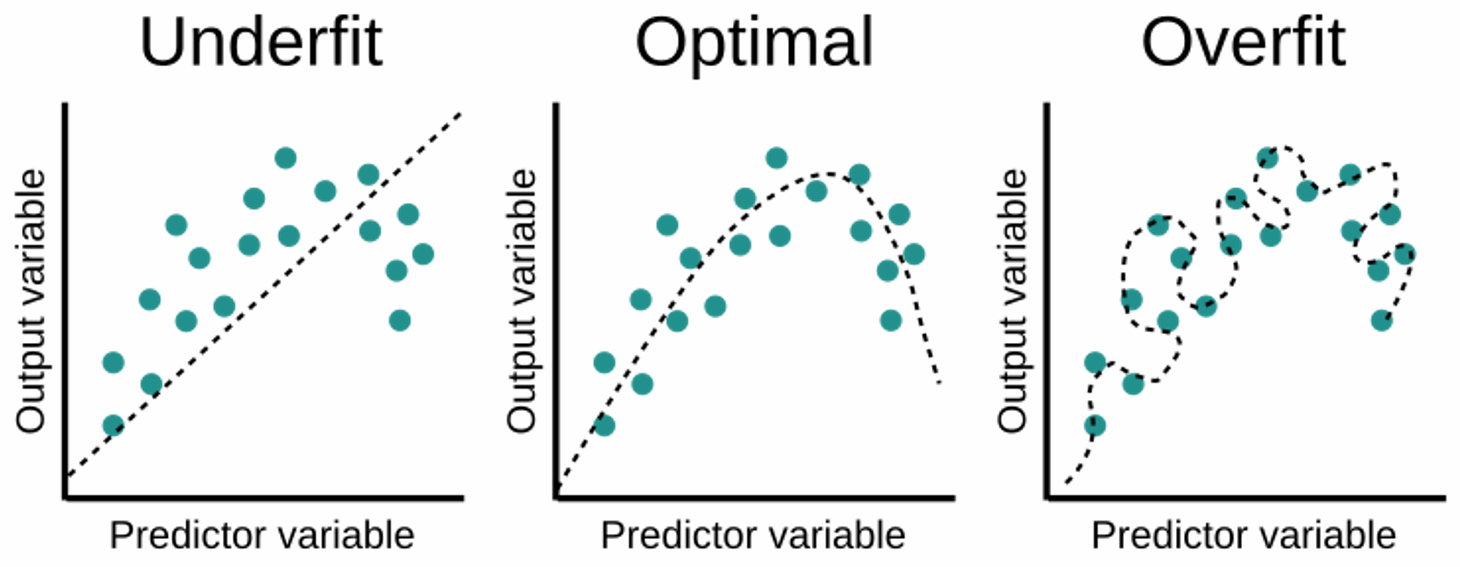
\includegraphics[width=0.95\paperwidth]{../static/course_3_img/overfit_underfit.PNG}}  
\end{frame}

\begin{frame}{Forecast Errors}

  \begin{block}{Definition: Forecast Errors}
    A forecast error is the difference between an observed value and its forecast

    \begin{equation*}
      e_{T+h} = y_{T+h} - \hat{y}_{T+h}|Y_T, \dots, Y_1
    \end{equation*}
  \end{block}

\medskip
  
\begin{wideitemize}
    \item The conditional set $Y_T, \dots, Y_1$ should only be taken from the training dataset
    \item The true value $y_{T+h}$ is taken from the test set
    \item Unlike residuals, forecast errors on the test involve multi-step forecasts
    \item These are the \textbf{true} forecast error, as the test data is not used to compute $\hat{y}_{T+h}$
  \end{wideitemize}
  
\end{frame}

\begin{frame}
  \frametitle{Example: Forecasting Beer Production}
     \makebox[\linewidth]{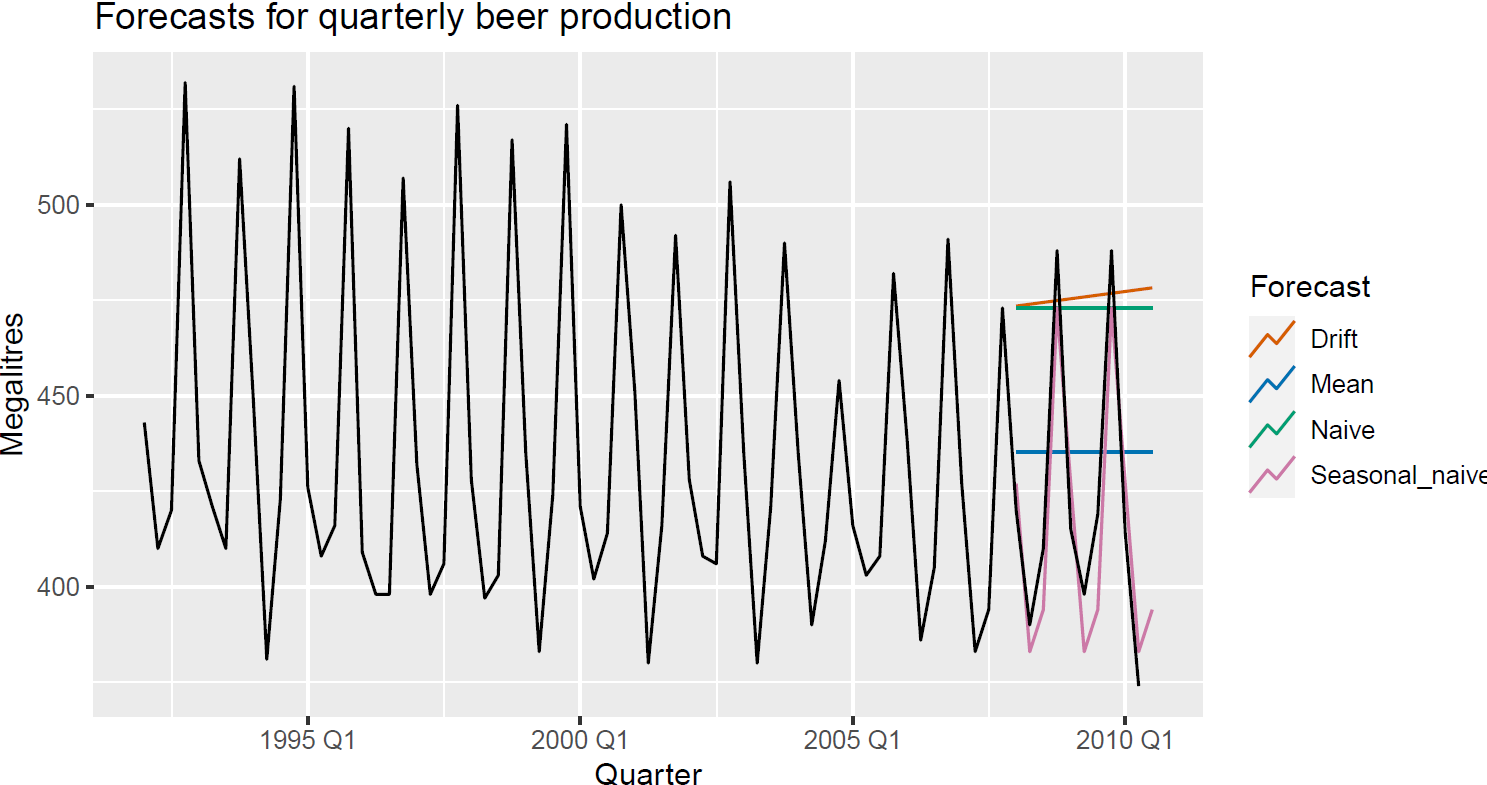
\includegraphics[width=0.95\paperwidth]{../static/course_3_img/beer_forecast.PNG}}  
\end{frame}

\begin{frame}{Measures of Forecast Accuracy}

  \begin{alertblock}{Main Metrics}
    \begin{wideitemize}
    \item \textbf{MAE}: mean absolute errors $\frac{1}{S}\sum_{s \in S} |e_{s, T+h}|$
    \item \textbf{MSE}: mean squared errors $\frac{1}{S}\sum_{s \in S} (e_{s, T+h})^2$
    \item \textbf{MAPE}: mean absolute percentage errors $\frac{1}{S}100*\sum_{s \in S} \frac{|e_{s, T+h}|}{|y_{s, t+h}|}$
    \item \textbf{RMSE}: root mean squared errors: $\sqrt{\frac{1}{S}\sum_{s \in S} (e_{s, T+h})^2}$
    \end{wideitemize}
  \end{alertblock}

  With:\\
  
  \begin{itemize}
  \item $y_{T+h}$: T+h observation, h being the horizon (h = 1, 2, ..., H)
  \item $\hat{y}_{T+h|T}$: the forecast based on data up to time $T$
  \item $e_{T+h} = y_{T+h} - \hat{y}_{T+h|T}$: The forecast errors
  \item $S$ is the testing sample
  \end{itemize}

  Note:\\
  \begin{itemize}
  \item MAE, MSE and RMSE are all \textbf{scale dependent}
  \item MAPE is scale independent but is only sensible if $y_t >> 0 \qquad \forall \ t$
  \item \textbf{Most commonly used: Time Cross-Validation with the lowest RMSE}
  \end{itemize}  
\end{frame}


\begin{frame}
  \frametitle{Time Series Cross-Validation}
     \makebox[\linewidth]{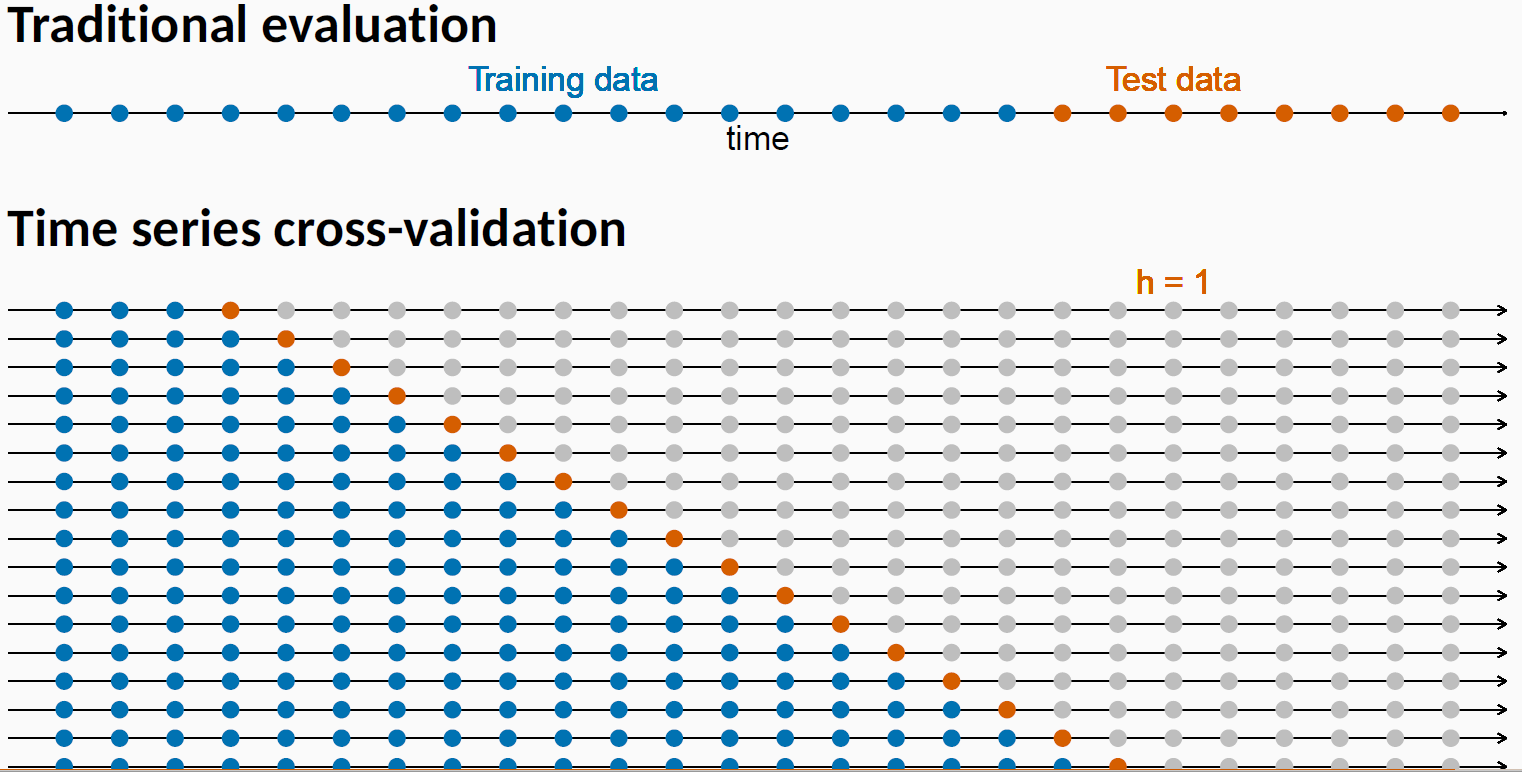
\includegraphics[width=0.95\paperwidth]{../static/course_3_img/time_series_cv_1.PNG}}  
  \end{frame}

\begin{frame}
  \frametitle{Time Series Cross-Validation}
     \makebox[\linewidth]{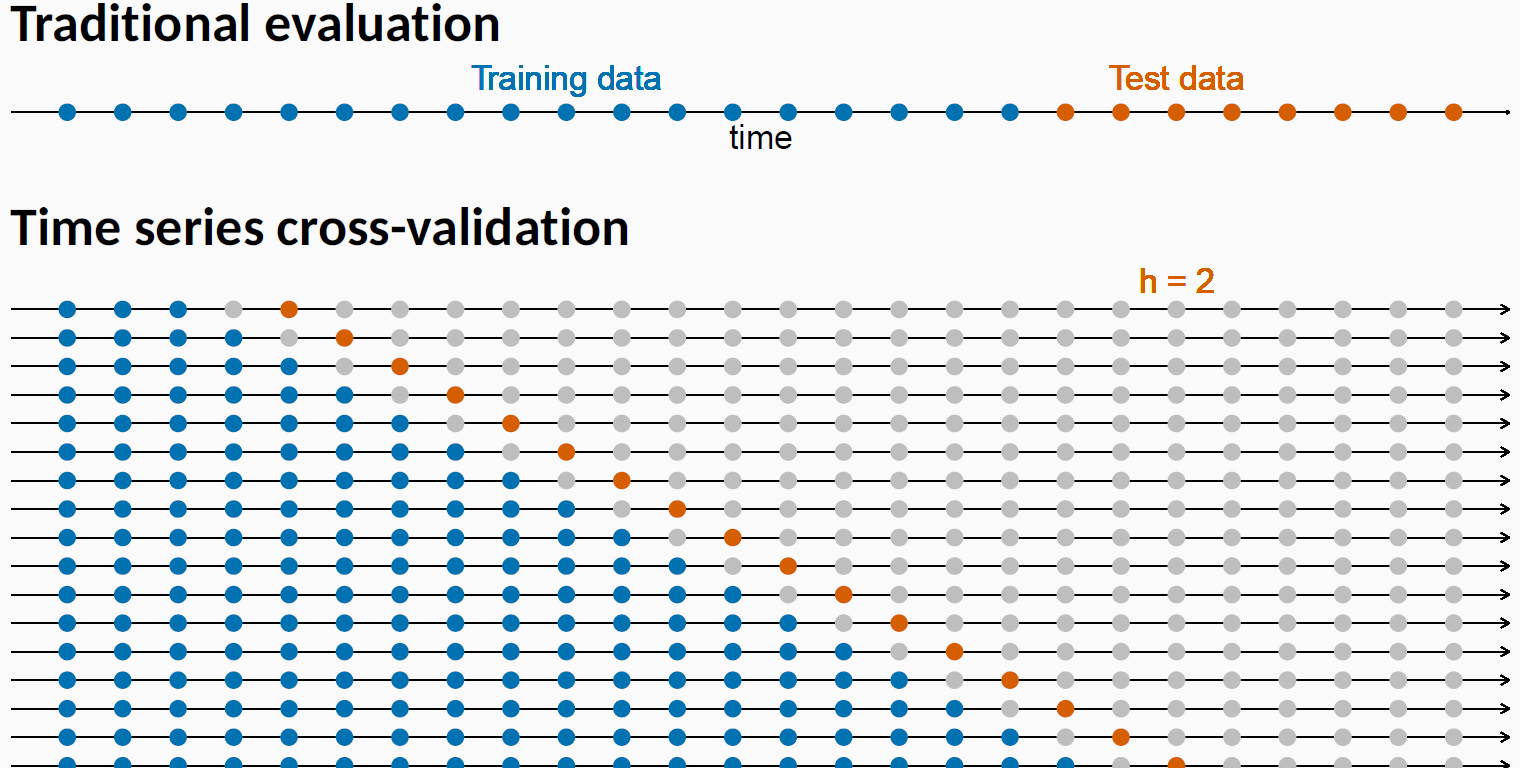
\includegraphics[width=0.95\paperwidth]{../static/course_3_img/time_series_cv_2.PNG}}  
  \end{frame}

\begin{frame}
  \frametitle{Time Series Cross-Validation}
     \makebox[\linewidth]{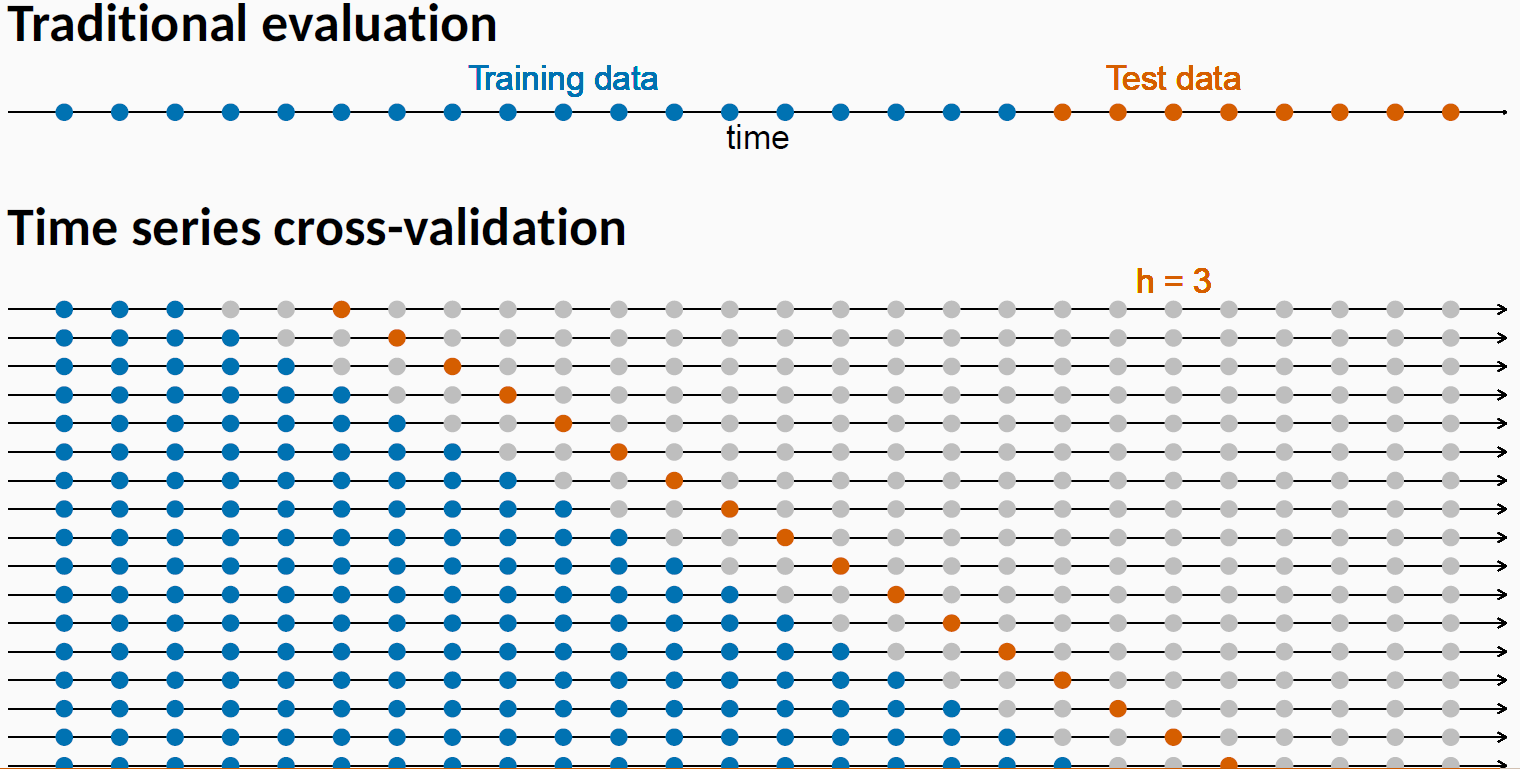
\includegraphics[width=0.95\paperwidth]{../static/course_3_img/time_series_cv_3.PNG}}  
  \end{frame}

\begin{frame}
  \frametitle{Time Series Cross-Validation}
     \makebox[\linewidth]{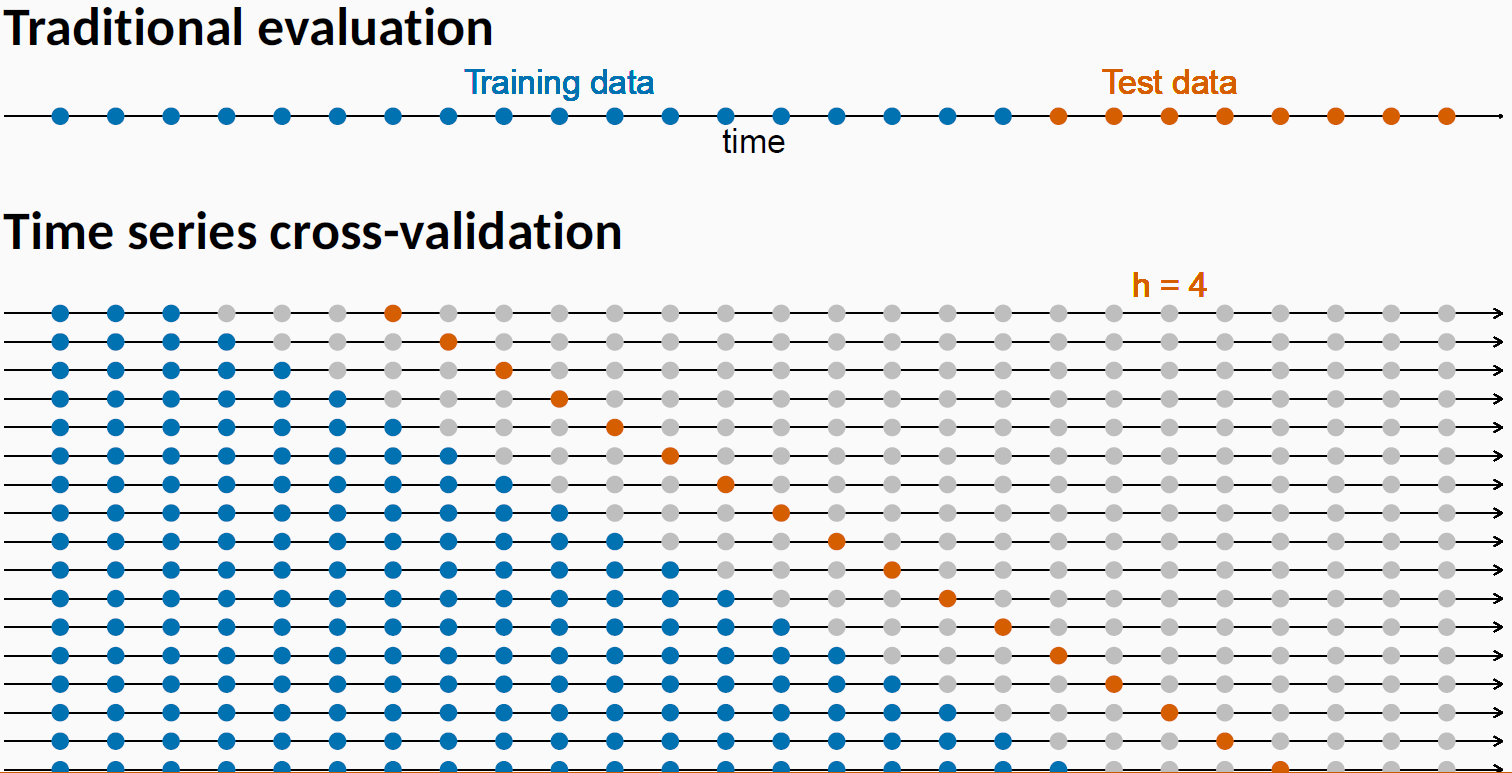
\includegraphics[width=0.95\paperwidth]{../static/course_3_img/time_series_cv_4.PNG}}  
  \end{frame}

\begin{frame}
  \frametitle{Time Series Cross-Validation}
     \makebox[\linewidth]{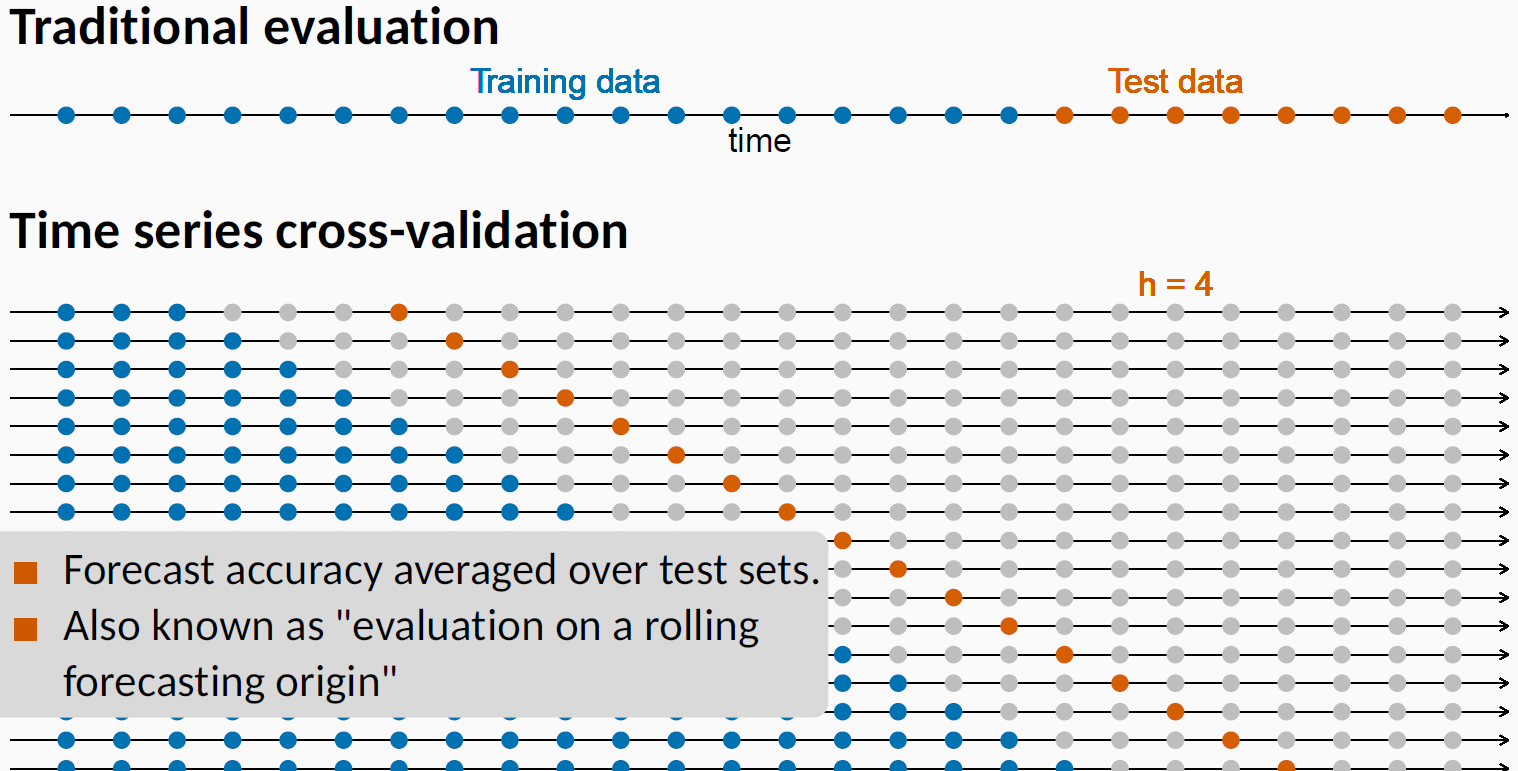
\includegraphics[width=0.95\paperwidth]{../static/course_3_img/time_series_cv_5.PNG}}  
  \end{frame}



  
  

%% ---------------------------------------------------------------------------
%% End document
%% ---------------------------------------------------------------------------
\end{document}






